\documentclass[a4paper,12pt]{article}
% Package imports
\usepackage{amsmath, amssymb, graphicx, hyperref, geometry, xcolor, listings, biblatex, tikz, algorithm, algorithmic, siunitx, multirow}
\geometry{margin=1in}
\addbibresource{references.bib} % Add a bibliography file

% Custom Commands
\newcommand{\R}{\mathbb{R}}
\newcommand{\dx}{\,\mathrm{d}x}

\begin{document}

% Title Section
\title{A Comprehensive \LaTeX{} Document Example}
\author{Your Name}
\date{\today}
\maketitle

\tableofcontents
\newpage

\section{Introduction}
This is an introduction to \LaTeX{} features. \LaTeX{} is great for writing technical and scientific documents.

\section{Mathematical Equations}
Here is an inline equation: \(E=mc^2\).

A displayed equation:
\begin{equation}
    \int_a^b f(x) \dx = F(b) - F(a)
\end{equation}

A matrix:
\begin{align}
    A &= \begin{bmatrix} 1 & 2 \\ 3 & 4 \end{bmatrix}
\end{align}

\section{Tables and Figures}
A simple table:
\begin{table}[h]
	\centering
	\begin{tabular}{|c|c|c|}
		\hline A & B & C \\ \hline 1 & 2 & 3 \\ 4 & 5 & 6 \\ \hline
	\end{tabular}
	\caption{A sample table}\label{tab:sample}
\end{table}

An example figure:
\begin{figure}[h]
	\centering
	\includegraphics[width=0.5\textwidth]{example-image}
	\caption{An example image}\label{fig:image}
\end{figure}

\section{Code Listings}
Here is some example code:
\begin{lstlisting}[language=Python, caption=Example Python Code]
def hello():
    print("Hello, World!")
\end{lstlisting}

\section{Algorithms}
An example algorithm:
\begin{algorithm}
	\caption{Example Algorithm}
	\begin{algorithmic}
		\STATE{}Initialize \(x=0\)
		\FOR{\(i=1\) to \(n\)}
		\STATE{}\(x = x + i\)
		\ENDFOR{}
		\STATE{}Return \(x\)
	\end{algorithmic}
\end{algorithm}

\section{Diagrams with TikZ}
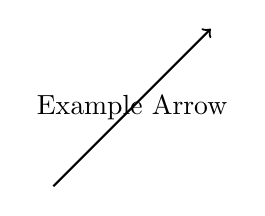
\begin{tikzpicture}
	\draw[thick,->] (0,0) -- (2,2);
	\node at (1,1) {Example Arrow};
\end{tikzpicture}

\section{Notations}
\textbf{Notations:} Some common mathematical notations include:
\begin{itemize}
    \item \textbf{Sets:} \(\mathbb{N}\) (natural numbers), \(\mathbb{Z}\) (integers), \(\mathbb{R}\) (real numbers)
    \item \textbf{Operators:} \(\sum_{i=1}^{n} i\), \(\prod_{i=1}^{n} i\), \(\lim_{x \to \infty} f(x)\)
    \item \textbf{Logic:} \(\forall x \in \mathbb{R}, \exists y \in \mathbb{R}\)
\end{itemize}

\section{Citations and References}
We cite an example source~\cite{exampleSource}.

\printbibliography[]

\end{document}
